\documentclass{article}
\usepackage[utf8]{inputenc}
\title{%
  \Huge{\textbf{Assignment-3}} \\ $ $\\
  \huge{\textbf{Ping Pong: A Networked Multi-Player Game}} \\ $ $ \\
  \textbf{\huge Team: SPYCODERS }}
\author{\Large{\textit{S}auhard Gupta \\ \texttt{2013ME10117}
\\$ $ \\ \textit{P}rabhu Prasad Panda \\ \texttt{2013ME10859}
\\$ $ \\ \textit{Y}ash Kumar Bansal \\ \texttt{2013ME10742}}}
\date{April 7, 2016}

\usepackage{natbib}
\usepackage{graphicx}

\begin{document}

\maketitle
\newpage
\tableofcontents
\newpage
\section{Introduction}
In this assignment, we intend to design and develop a networked \textbf{\textit{multi-player Ping-Pong game}} that can be played on a desktop machine.
\newline
\newline
\textbf{Game description:}
\newline
The game has \textbf{maximum four players} where each player \textit{guards his/her wall }from the ball. If the \textbf{ball touches the player’s wall 3 times}, the player is deemed as \textbf{dead} and \textbf{his/her paddle is removed} from the game board. This is a continuous action game; even if a player misses the ball, the ball continues to move on the game board. Some players in the game can be \textbf{manual}, and others can be backed by the \textbf{computer} (different difficulty levels: easy/medium/hard). \textbf{The player who remains alive at the end of the game is deemed as the winner}. There can be \textbf{multiple balls} which moves in a random direction at the start of the game. 
\newline
\newline
\textbf{Connection:-} Here is how different players play against each other;
\begin{enumerate}
\item \textbf{Single player:} If there’s only one manual player, he/she has to play against computer players on his/her local machine.  
\item \textbf{Multi-player:}In this case, \textit{one player starts the game, and others join the game by providing the IP of the starting machine}. The IP's of all machines involved in the game will be exchanged at this time. Once started, the game is completely peer-to-peer, meaning there is no central server. 
\end{enumerate}
Here is how a simple 4-player Ping-Pong would look like:
\newline
\begin{figure}[h!]
    \centering
    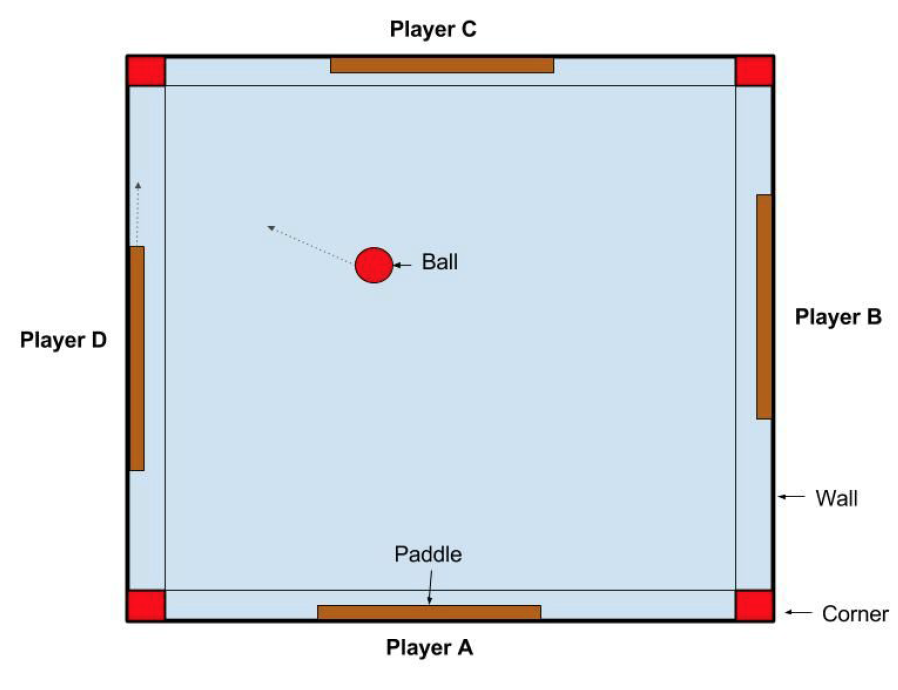
\includegraphics[width=.5\textwidth]{game_board}
    \caption{Representative Game Board}
\end{figure}
\section{Scope of the Game}
\subsection{Multiple Balls and other features}
\begin{itemize}
\item \textbf{Multiple Balls:} Our plan is to allow the players to select the number of balls before the start of the game. This ranges from 1 to 4. The balls will appear at the centre of the board symmetrically and after the starting timer blows off. They will be directed arbitrarily towards the players (but it will be ensured that not more than one ball is directed towards any player). The number of the balls can change during the course of the game, if the players gains any special powers, this will be explained in the respective section. The dynamic number of balls can be at maximum 8 an
\item \textbf{Timer:} In the beginning of the game in order to the allow every player to settle down, we will have a timer 3 $\to$ 2 $\to$ 1.
\item \textbf{Multiple Backgrounds and Associated Properties:} The game allows the players to change the board. The various boards apart from having different backgrounds also have different values for properties. The boards to be included are:-
\begin{enumerate}
    \item Grass turf
    \item Clay-turf
    \item Hard-turf
    \item Synthetic-turf
\end{enumerate}
The aim of different turfs is to have different background affects and different background colors.
\item \textbf{Speed Control of Ball:} The initial speed of the ball will be set by the player as Setting of the game. With every collision of the ball with the bat, the speed of the ball increases by x\%, where x can be changed by the players.

\end{itemize}
\subsection{Acquirable Special Players}
During the course of the game the player can gain some special power if the ball deflected by their bat manages to hit the pop ups for these powers. The \textit{SPECIAL POWERS} include:
\begin{enumerate}
    \item \textbf{Bat}
    \begin{enumerate}
        
    \item \textbf{Double Length Of the Bat:-} In this mode the length of the bat doubles, thus acting as an advantage for the user. 
    \item \textbf{Half The Length:-} In this mode the length of the bat ha;ves, thus acting as an disadvantage for the user. 
    \item \textbf{Chop Mode:-}In this mode the ball will get deflected at an increased speed of X times (X yet to be decided). This increased speed will continue till it hits the wall or the bat of another user. This acts as an advantage for the player.
    \item \textbf{Serve Mode:-} In this mode the bat is able to grab the ball and serve at a speed that is decided by the a bar. 
    \item \textbf{Extra Life:-} In this mode the player gets an extra life if the ball on deflection from his/her bat hits the \textit{EXTRA LIFE} pop out.
    \end{enumerate}
    
    \item \textbf{Screen Powers}

    \begin{enumerate}
        
    \item \textbf{Nitro-Boost Mode: }In this mode the ball will get deflected at an increased speed of X times (X yet to be decided). This increased speed will continue for next 15 seconds.
    \item \textbf{Tortoise Mode: }In this mode the ball will get deflected at an reduced speed of X times (X yet to be decided). This reduced speed will continue for next 15 seconds.
    \item \textbf{Split Ball: }In this mode the ball will split into two halves and the two halves will get deflected at random directions. This power will on come if the current number of balls are less than 8.
    \item \textbf{Black Hole: }In this mode the ball will be consumed at the black hole. This power will be available only if the current number of balls are greater than 1.
    \item \textbf{Warp Hole: }In this mode the ball will disappear from a point in the board and appear from another.
    
    \end{enumerate}
\end{enumerate}}
\section{Physics of the Game}

\subsection{Dynamic parameters of ball and paddles}
Following variables shall be tracked/evaluated during rendering of the game:
\begin{itemize}
    \item Number of active players and balls in the system.
    \item For each ball:
    \begin{itemize}
        \item position of centre (x,y)
        \item velocity of centre ($v_x$,$v_y$)
        \item angular velocity ($\omega$)
    \end{itemize}
    \item For each paddle:
    \begin{itemize}
        \item orientation of the paddle (identifier of the paddle)
        \item position of centre of paddle (x)
        \item velocity of paddle (v)
        \item acceleration of paddle (a)
    \end{itemize}
\end{itemize}
\subsection{Collisions between bodies}

Following are the types of collisions that can occur in the game:
\begin{itemize}
    \item between ball and bat
    \item between two balls
    \item ball hitting a corner
\end{itemize}

\begin{figure}[h!]
    \centering
    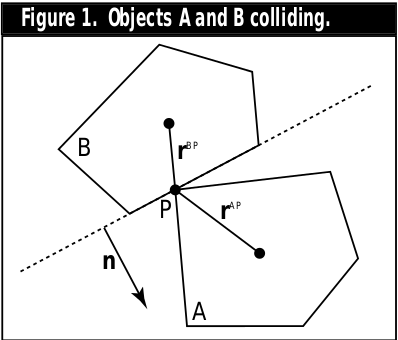
\includegraphics[width=.5\textwidth]{collision.png}
    \caption{Collision between two bodies}
    
\end{figure}
The physics for handling collisions is as follows$^\citep{collisionphysics}$:\\
Suppose objects A and B collide with each other at point P.
Let the position vector of point P with respect to centre of masses of two objects be $r^{AP}$ and $r^{BP}$, initial velocities of bodies be $v_1^A$ and $v_1^B$ and angular velocities be $\omega_1^A$ and $\omega_1^B$, respectively.\\
Then the parameters after collision can be computed using following formulae:
\begin{itemize}
    \item $v^{AB} = v^{AP} - v^{BP}$\\
    \item n is a vector normal to plane of collision pointing towards A \\
    So, if object A is circular, then $n = r^{AP}$
    \item $v_2^{AB}\cdot n = -ev_1^{AB}\cdot n$ where e is the coefficient of restitution.\\
    \item $v_2^A = v_1^A + \frac{J}{M^A} \cdot n$
    \item $w_2^A = w_1^A + \frac{r_\perp^{AP}\cdot Jn}{I^A}$
    \item $v_2^B = v_1^B - \frac{J}{M^B} \cdot n$
    \item $w_2^B = w_1^B - \frac{r_\perp^{BP}\cdot Jn}{I^B}$
    \item where J, the impulse imparted to object A by object B, is given by \\$J = \frac{-(1+\epsilon)v_1^{AB}\cdot n}
    {n\cdot n (\frac{1}{M^A}+\frac{1}{M^B}) + \frac{({r_\perp^{AP}\cdot n})^2}{I^A} + \frac{({r_\perp^{BP}\cdot n})^2}{B^A}}$
\end{itemize}
Calculating J and hence the final velocities will give desirable results.

\subsection{Simulating motion of bat from keyboard input}

The key pressed by user has to be converted into corresponding movement of the paddle. Practically we have to control position and velocity of the paddle. So, we can set a constant acceleration($a_r$) while the key is pressed, subject to a cutoff speed. Once the key is released, the paddle would decelerate rapidly till it stops or some other key is pressed. Typically, the paddle would move till about 0.5 seconds after key is released, to give it a more realistic effect.

\subsection{Motion of ball on the board}
We assume that there is no friction between the ground and the ball to avoid slowing down of the ball, as it will lower the game play.

\section{Computer Player}
The computer player can play in three modes: easy, medium and hard. We have also planned to have a legendary mode in which the computer player can never lose. 

\subsection{Algorithm of the Computer Player}
The motion control will be done by calling two functions only - LeftButtonPress() and RightButtonPress(). These functions will simulate the behaviour of the bat as if an user is controlling them and has pressed the left or the right button.
\begin{itemize}
    \item \textbf{Easy Player:} In the easy player, the computer player will try to move towards the ball having the smallest y-coordinate. The LeftButtonPress() or RightButtonPress() will be called so long as the x-coordinate of the ball is outside the acceptable neighbourhood of the x-coordinate of the centre of mass of the bat. 
    \item \textbf{Medium Player}: A medium player will be sensitive to the ball only when it feels that the ball is approaching it and accordingly it will calculate the position at which the ball will arrive at its end and try to reach there. In case of multiple balls being directed towards the computer player, it will be sensitive to the one which will land first. Whenever the computer player is not ball sensitive, it will just move left/right randomly.
    \item \textbf{Hard Player}:In the hard player case, the computer player calculates the expected time for all the balls for landing at its place and becomes sensitive to the one with the least expected landing time. It computes the expected landing position of this ball and places itself at that position. This gets updated after every collision.
    \item \textbf{Legendary Player}: As for yet, we have not thought of any algorithm for this. We will implement this only after the game is complete so that we are well aware of the ranges of the speed and direction of the ball after being hit by a bat or collided by a ball and hence prepare the bat accordingly to handle this.
\end{itemize}
\subsection{Where does the Computer Player run?} As the location of the computer player is not entirely theoretically calculable and involves randomness, we need to send information about its location and velocity to other machines time-to-time. For this purpose, we have a priority queue of local machines. The computer players will run on the machine with highest priority. The co-ordinates and velocity of the computer controlled bat will be sent to other users from time-to-time(most probably after every time the co-ordinate changes) so that the other local machines are able to precisely display the computer player. When the connection of the highest priority machine goes out, the next highest priority machine controls the computer players from the latest information it had about them.  
\subsection{Handling of events by the computer player}
\begin{itemize}
\item \textbf{Sending bat info to other machines}: Every time, the bat's co-ordinates, velocity or button pressed(left ,right or nothing) changes, this information is sent to other local machines so that these machines could have the latest information about the bat.
\item \textbf{Connection Out Handling}: If the connection of the controlling machine goes out, the control is transferred to the machine with the next highest priority. This machine resumes operation from the latest information it has about the machine. So this highlights the importance of sending velocity and other parameters apart form co-ordinates at every stage to other machines. Ideally only co-ordinates need to be transmitted for display in other machines. But in order to handle the cases of connection failure, we need to send the entire information so that another machine can resume the control operation.
\end{itemize}
\section{Network Communication}
\subsection{Information exchanged between different machines}
As we are having peer-to-peer connection, there is no one server in our case. Hence as explained in the section of computer player, we will have a priority queue of local machines. So all the events taking place in the game which are not specific to a particular player, will be controlled by the local machine with the highest priority and on the occasion of an event, it will send the required information to the other local machines, so that they can update their view accordingly and be in a position to take control of the game when the controller machine goes out of connection. For events which are player linked like movement of bat or striking of ball, the associated machine sends the required information to other machines for local updation. Let's take a look at some of the events and the information exchange associated:
\begin{itemize}
    \item \textbf{A local machine moves his bat:} In this case the co-ordinates of the bat and the velocity and the key-press states are transmitted to the other local machines. As mentioned earlier in the section under Computer players, for purposes of display only the co-ordinates are required but in order to resume the game of that player as a computer player once the connection is lost other parameters are required as well.
    \item \textbf{A local machine hits a ball:} In this case the status of the ball, i.e., if any special attribute gets associated with it etc. are transferred in addition to the position and velocity of the ball. The transfer takes place from the hitting local machine to others. A similar information is transferred when the player is unable to hit and loses a life.
    \item \textbf{Appearance of special powers:} These are randomly generated by the controller machine and get transmitted to other local machines.
\end{itemize}
\subsection{Ensuring that all players must see the same game state}
It is somewhat obvious that the game needs to have a global clock to handle events(track inputs, change of co-ordinates of bat or ball etc). We plan to use this clock similar to a flip-flop that is the event is tracked only once in a clock cycle. So to ensure proper synchronisation, we must ensure that the cycle time of the clock is much larger than the network delay of transmitting information. As the state of the game changes only once in each clock cycle, this will ensure that all the local machines are in the same state the next time the clock becomes active.
\subsection{Event Flow for Network Message}
As we have used peer-to-peer connection, the event flow basically involves sending the necessary information to the peers at each clock cycle. 
\newline
\begin{figure}[h!]
    \centering
    \includegraphics[width=.5\textwidth]{Network_Transfer_Flowchart}
    \caption{Flowchart showing transfer of messages via network}
\end{figure}
\subsection{Checking for local machine disconnection:-}
To ensure a hassle free gaming experience, we would have an connection message sent between every pair of players, once in every clock cycle. In case any local machine does not receive this message, then such a machine would be classified disconnected and handled accordingly.
\subsection{On disconnection}
In case any machine(M) is classified as disconnected, the local machine will wait for 5 clock cycles(5 is an approximate value that could be changed depending on the quality of connection) before replacing M by a computer player, whose level was specified before start of the game. In the 5 clock cycles, please respond messages will be send by the local machine to M, and if during this period, any response is received then M's game resumes owtherwise the computer player takes guard.


\bibliographystyle{plain}
\bibliography{references}
\end{document}
